\section{Methodology and Experiments}

The T-Hex kit, as the name suggests, is originally a hexapod. However, due to hardware failures present in our kit, the two middle legs had to be taken out, making it a quadruped. As we wish to eventually extend this work on hardware, we treated the robot as a quadruped. Going forth, T-Hex refers to this quadruped version of the original kit as seen in figure \ref{fig:tquad}. 

\begin{figure}[h]
    \centering
    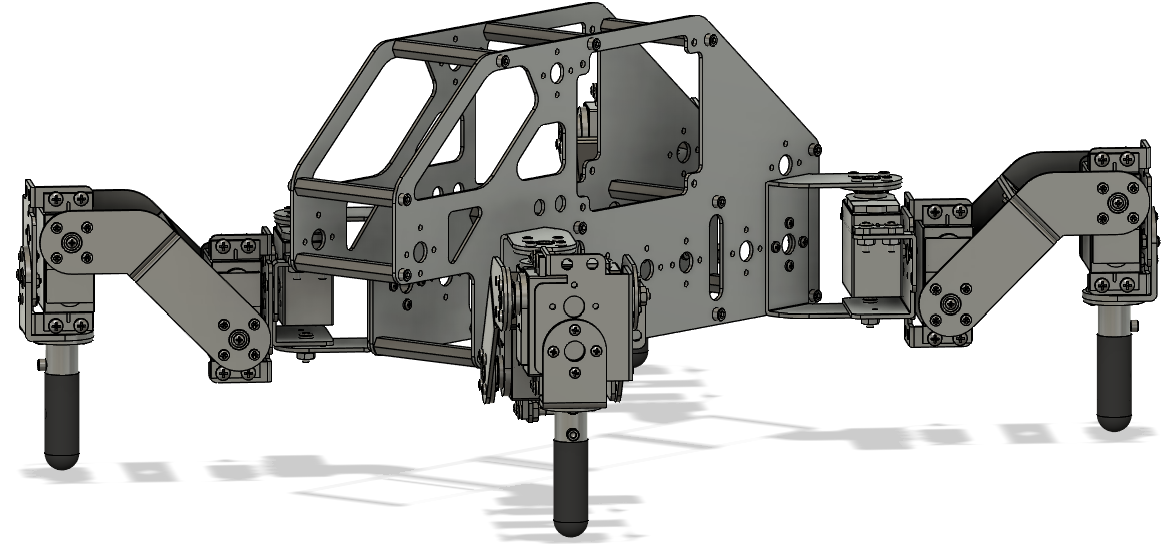
\includegraphics[width=0.7\linewidth]{tquad.png}
    \caption{T-Hex (as seen in SolidWorks) with its middle legs removed, making it a quadruped.}
    \label{fig:tquad}
\end{figure}

\subsection{Kinematics}

The motors of the T-Hex take position commands, that is what angle they should move to, as opposed to torque commands which are common in high-end motors \cite{bledtMITCheetah32018, hutterANYmalHighlyMobile2016}. Each leg of T-Hex has 3 motors (or joints), at the hip, knee, and ankle. Many locomotion controllers, such as an open-loop kinematic gait, output the position of the foot, that is the end point of the legs, at any given time. The problem of determining what joint positions result in a desired foot position is known as the Inverse Kinematics (IK) problem. Solving the IK of a legged robot is well-established. Using the Denavit-Hartenberg (DH) convention, frames of reference are assigned across the robot's legs and the homogenous transform matrices can be multiplied to obtain equations that take in joint positions and output resulting foot positions, known as the Forward Kinematics (FK) equations. The FK equations can then be used to derive the IK equations, that take in foot positions and output the corresponding joint angles. A detailed derivation is omitted for the sake of brevity, but a similar derivation can be found in \cite{sunHexapodRobotKinematics2017}. The IK equations for our robot are as follows:
\begin{align}
    \theta_1 &= \text{atan2}(y, x) \\
    \theta_2 &= 
    \begin{cases} 
        \arcsin\left(\frac{z}{a_2}\right) + \phi_2 & \text{for right legs} \\
        \arccos\left(\frac{z}{a_2}\right) - \phi_2 & \text{for left legs}
    \end{cases} \\
    \theta_3 &= 
    \begin{cases} 
        \frac{\pi}{4} & \text{for right legs} \\
        -\frac{\pi}{4} & \text{for left legs}
    \end{cases} \\
    \theta_4 &= 
    \begin{cases} 
        \phi_1 - \arcsin\left(\frac{\Psi}{a_1}\right) & \text{for right legs} \\
        -\arccos\left(\frac{\Psi}{a_1}\right) - \phi_1 & \text{for left legs}
    \end{cases} 
\end{align}

where $\Psi, a_1, \phi_1 a_2,$ and $\phi_2$ are defined as:
\begin{align}
    \Psi &= \frac{1}{2L_4} \Big[ (x \cos\theta_1 + y \sin\theta_1 - L_1)^2 + z^2 \notag \\
    &\quad - L_2^2 - L_3^2 - L_4^2 - 2L_2 L_3 \cos\theta_3 \Big] \\
    A_1 &= L_2 \cos\theta_3 + L_3 \\
    B_1 &= L_2 \sin\theta_3 \\
    a_1 &= \sqrt{A_1^2 + B_1^2} \\
    \phi_1 &= 
    \begin{cases} 
        \text{atan2}(A_1, B_1) & \text{for right legs} \\
        \text{atan2}(B_1, A_1) & \text{for left legs}
    \end{cases} \\
    A_2 &= L_2 + L_3 \cos\theta_3 + L_4 \cos(\theta_3 + \theta_4) \\
    B_2 &= L_4 \sin(\theta_3 + \theta_4) + L_3 \sin\theta_3 \\
    a_2 &= \sqrt{A_2^2 + B_2^2} \\
    \phi_2 &= 
    \begin{cases} 
        \text{atan2}(B_2, A_2) & \text{for right legs} \\
        \text{atan2}(A_2, B_2) & \text{for left legs}
    \end{cases}
\end{align}

where $x, y,$ and $z$ are input foot coordinates in the \textit{hip frame} of the leg and $L_i$ indicates the length of the $i$-th link. While each leg in the T-Hex has only 3 motors, it has a $45$ degree bend in between the knee and ankle motors (as can be seen in figure \ref{fig:tquad}) which we model as a rigid joint (see eq. (3)); hence, we have four links.


\subsection{Simulation}

To simulate the robot, we used the available CAD model (as seen in figure \ref{fig:tquad}) and the SolidWorks plugin SW2URDF \cite{Sw_urdf_exporterROSWiki} to export a URDF file for simulating the robot. Certain properties, such as mass and inertia, were exported incorrectly and had to be manually adjusted using calculations from SolidWorks. Furthermore, we also made a simplified collision mesh to be used in place of the high fidelity CAD model to speed up simulation. We used Gazebo Sim as our primary simulator.

To simulate terrain, we had two types of terrains: a flat world with some narrow passageways and crawl spaces made out of cuboids, and a rough terrain cave procedurally generated via modifying PLUME \cite{garciaPLUMEProceduralLayer2025}, a procedural cave generation framework, for our lava tube case. In both terrains, the ground's friction coefficient was set to 0.7.

\begin{figure}[h]
    \centering
    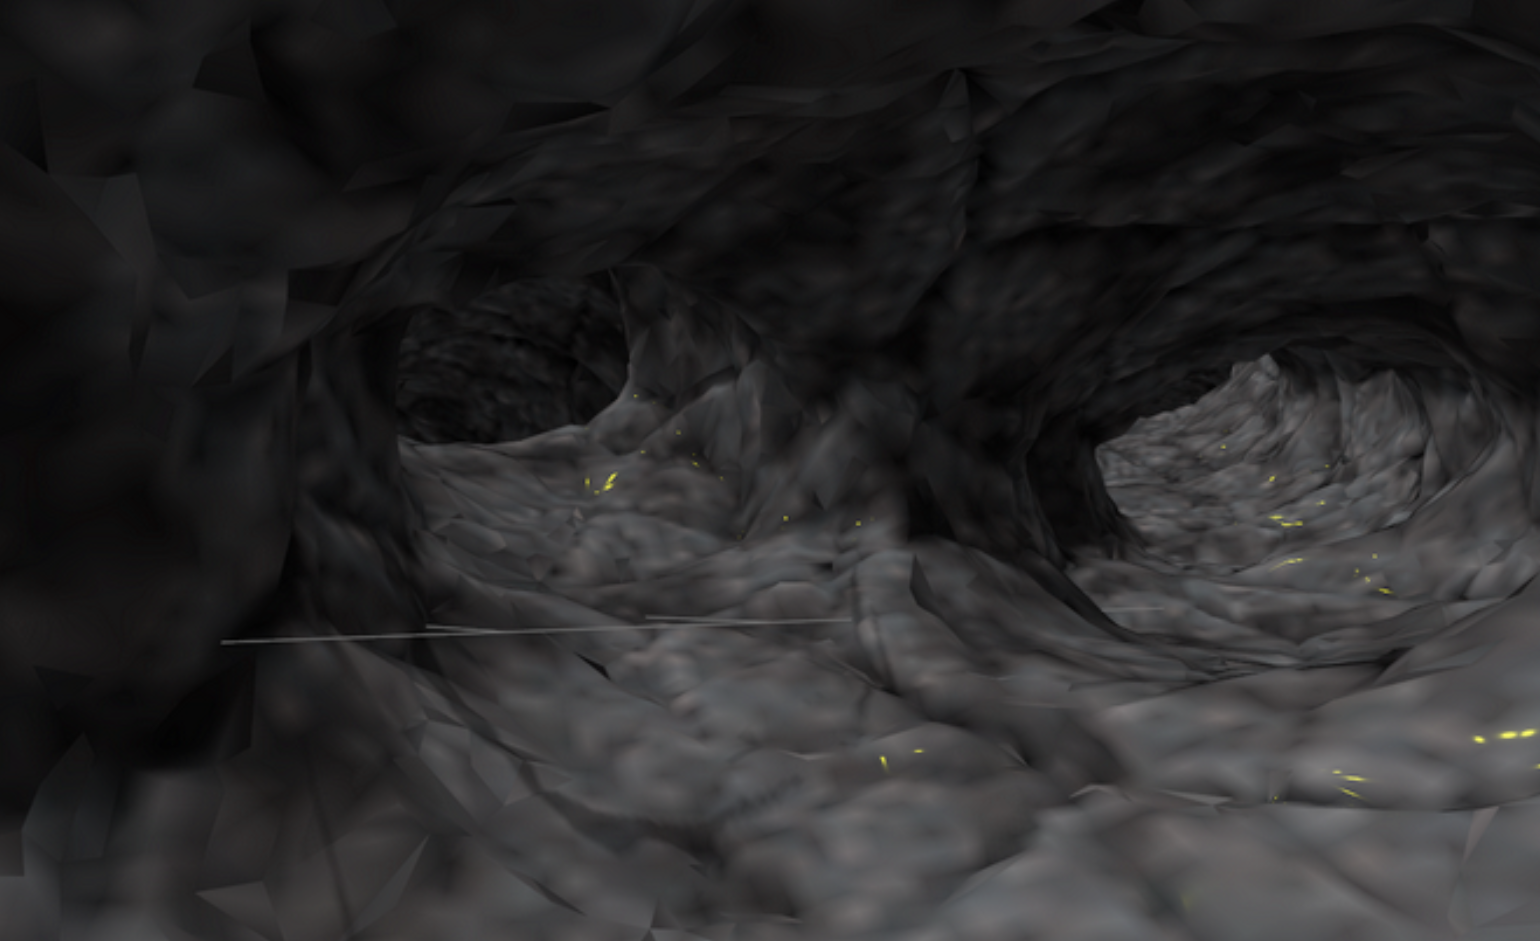
\includegraphics[width=0.8\linewidth]{cave.png}
    \caption{Interior of cave generated using PLUME \cite{garciaPLUMEProceduralLayer2025}}
    \label{fig:cave}
\end{figure}

After simulating the robot and terrains to test our locomotion controllers in, we set out to work on the locomotion controllers themselves. To cover both model-free and model-based controllers, we worked on the following three controllers:
\begin{enumerate}
    \item An \textbf{open-loop kinematic gait} to serve as a baseline for walking in flat terrain
    \item A \textbf{deep reinforcement learning} based controller trained in Isaac Lab 
    \item A \textbf{model-based controller} based off of MIT Cheetah 3's locomotion controller \cite{bledtMITCheetah32018}
\end{enumerate}

In simulation, the work on perception was taken separately, with the goal of giving posture signals that could be sent to the above controllers. 

\subsection{Open-loop kinematic gait}

For this controller, we use a crawl gait. For a quadruped, a crawl gait is one where at most one leg is in swing phase at a given time, giving a wider support polygon under the robot with three legs in stance. Hence, the stance phase is three times longer than the swing phase. The different permutations for the swing legs may result in better or worse stability. Typically, alternating sides (left and right) in the swing order helps keep the robot from tilting too far on one side. A possible schedule is given in table \ref{tab:crawl_gait}. 

\begin{table}[h]
    \centering
    \caption{Crawl Gait Schedule}
    \label{tab:crawl_gait}
    \newcolumntype{Y}{>{\centering\arraybackslash}X} 
    
    % \columnwidth ensures it spans exactly the width of the IEEE column
    \begin{tabularx}{\columnwidth}{@{}lYYYY@{}}
        \toprule
        \textbf{Leg} & \textbf{$0 \le t < \frac{N}{4}$} & \textbf{$\frac{N}{4} \le t < \frac{N}{2}$} & \textbf{$\frac{N}{2} \le t < \frac{3N}{4}$} & \textbf{$\frac{3N}{4} \le t < N$} \\
        \midrule
        FR & \cellcolor{white} Swing & \cellcolor{gray!30} Stance & \cellcolor{gray!30} Stance & \cellcolor{gray!30} Stance \\
        BL & \cellcolor{gray!30} Stance & \cellcolor{white} Swing & \cellcolor{gray!30} Stance & \cellcolor{gray!30} Stance \\
        BR & \cellcolor{gray!30} Stance & \cellcolor{gray!30} Stance & \cellcolor{white} Swing & \cellcolor{gray!30} Stance \\
        FL & \cellcolor{gray!30} Stance & \cellcolor{gray!30} Stance & \cellcolor{gray!30} Stance & \cellcolor{white} Swing \\
        \bottomrule
    \end{tabularx}
\end{table}


We pre-compute trajectories of $N$ discrete foot positions for each leg. A normalized phase variable $\tau \in [0, 1]$ dictates how far along a leg is in either swing or stance phase (based on the gait schedule). In swing phase, a quadratic bezier curve is used to generate trajectory points whereas in stance phase, linear interpolation between the start and end points of the swing phase can be used.

\begin{align}
    \mathbf{p}_{swing}(\tau) &= 
    \begin{bmatrix} 
        X \\ 
        (1-\tau)^2 P_{y} + 2(1-\tau)\tau Q_{y} + \tau^2 R_{y} \\ 
        (1-\tau)^2 P_{z} + 2(1-\tau)\tau Q_{z} + \tau^2 R_{z} 
    \end{bmatrix} \\
    \mathbf{p}_{stance}(\tau) &= 
    \begin{bmatrix} 
        X \\ 
        \frac{T}{2} (1 - 2\tau) \\ 
        S 
    \end{bmatrix}
\end{align}

where $X$ is the longitudinal distance from the hip (the sprawl of the robot), $S$ is the vertical distance from the hip (how far above the ground the robot stands), $T$ is the total distance covered in the stance phase, and $P = [X,-T/2, S]^T, Q = [X,0, S + 2A]^T,$ and $R = [X,T/2, S]^T$ are the control points of the bezier curve, where $A$ is the amplitude of the swing phase (how far above the ground is the apex of the swing). To make the generated trajectories parallel to the length of the robot, the trajectories for each leg were rotated by the angle corresponding to the offset of the corresponding hip frame in zero position (the hip motor at zero degrees) from the frame placed at the center of the robot.

\begin{figure}[h]
    \centering
    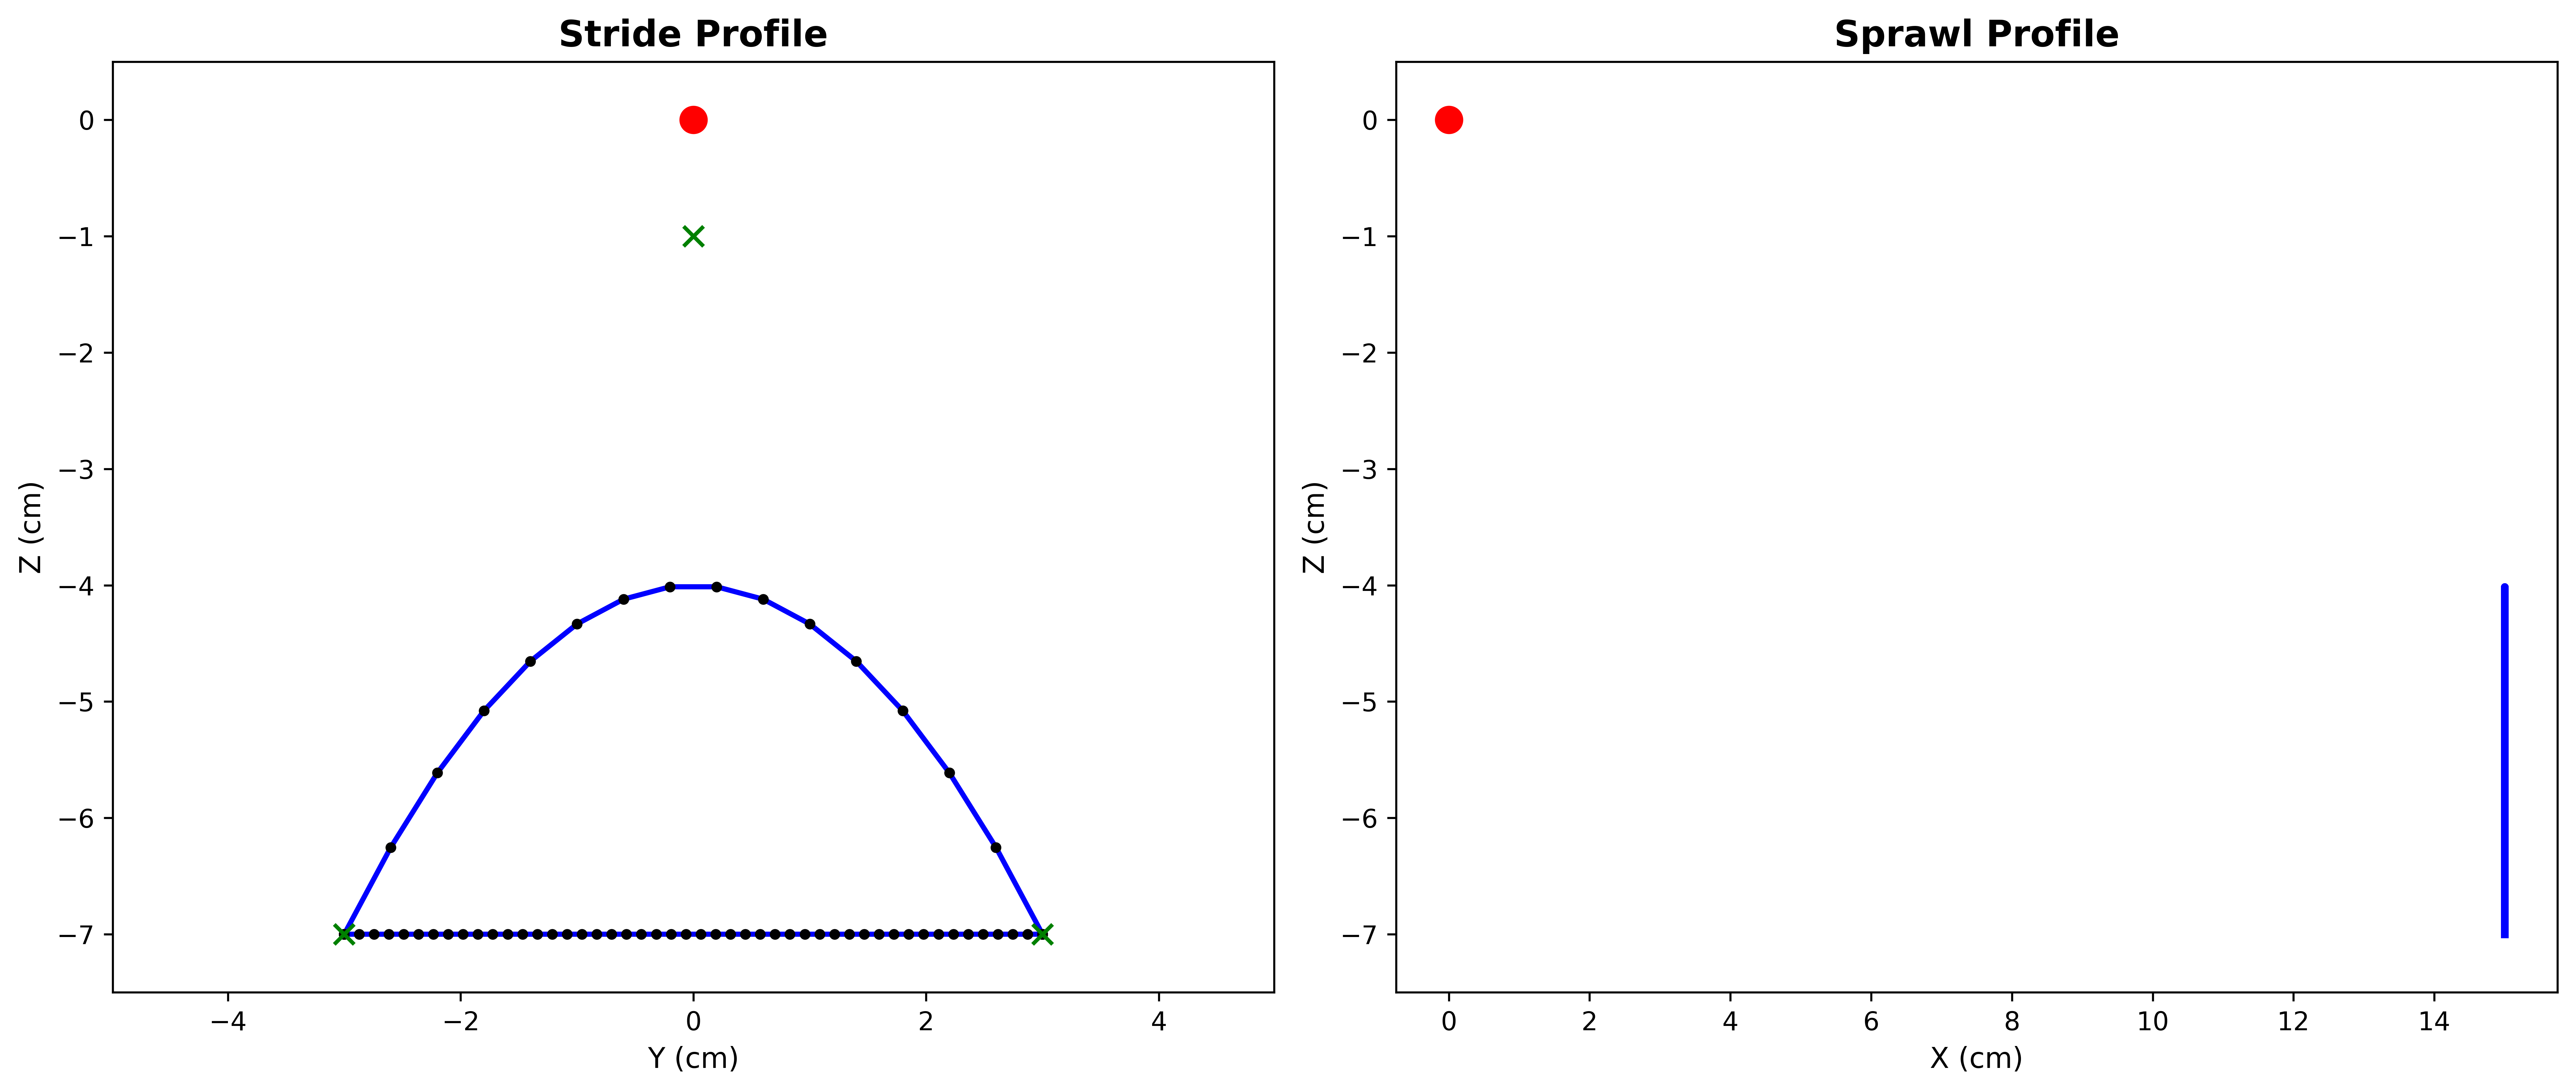
\includegraphics[width=\linewidth]{foot_trajectory_combined.png}
    \caption{Visualization of Bezier Curve with $N = 64, X = 15, S = -7, A = 3, T = 6$ in the hip's Y-Z plane (left) and X-Z plane (right). The red point indicates the location of where the hip frame was placed. The green crosses (in the left plot) indicate the bezier curve control points $P$, $Q$, and $R$.}
    \label{fig:gait}
\end{figure}

\subsection{Deep Reinforcement Learning-based Controller}

To train a DRL-based controller, we used Isaac Sim to convert the robot's URDF into an USD file. Then, we used a pre-existing Isaac Lab setup for velocity tracking for ANYmal C and modified it for our use case. 4096 instances of T-Hex \footnote{Other hyperparameters were kept the same as \cite{rudinLearningWalkMinutes2022}} were spawned in an environment containing three different categories of terrains: random noise rough terrain created using grids of points of varying heights connected together with planes, random blocks rough terrain consisting of flat blocks of varying heights arranged in a grid, and random inclines created by taking the maximum and minimum of planes of varying slopes. The maximum vertical distance between any two points in the random noise rough terrain was set to 6cm, the maximum vertical distance between adjacent blocks in random blocks rough terrain was set to 3cm, and the slope of the planes in random inclines was between -15 and 15 degrees. However, as is typical in literature \cite{rudinLearningWalkMinutes2022, rudinAdvancedSkillsLearning2022, hoellerANYmalParkourLearning2023}, instead of spawning all robots at the highest end of the difficulty for each category, a curriculum learning approach was adopted where the robots would spawn in easier difficulty variants of each category, and advance to higher difficulties after successfully performing at the lower difficulty. Further details regarding the setup can be found in \cite{rudinLearningWalkMinutes2022}.

The input to the policy network was the robot's current joint positions, the projected gravity vector (the gravity vector in robot's base frame), its angular velocity, previous actions given by the policy, and the user commands for $xy$-linear velocity and $z$-angular velocity (yaw rate). The network's output was joint commands for each of the twelve joints. The value network was given all the same inputs as the policy network, along with some privileged information to speed up training, such as joint velocities, robot's base linear velocity, and the height values of 128 random points on the terrain around the robot.

Table~\ref{tab:rl_rewards} lists the rewards and penalties used during training along with their weights.

\begin{table}[h!]
    \centering
    \caption{Rewards and Penalties for Training DRL-based Controller}
    \label{tab:rl_rewards}
    % \newcolumntype defines a centered X column to stretch the math evenly
    \newcolumntype{C}{>{\centering\arraybackslash}X}
    \begin{tabularx}{\columnwidth}{@{} >{\raggedright\arraybackslash}p{2.8cm} C c @{}}
        \toprule
        \textbf{Reward/Penalty} & \textbf{Calculation} & \textbf{Weight} \\
        \midrule
        XY-Linear Velocity Tracking & $\exp\left(-\frac{\|\mathbf{v}_{xy} - \mathbf{v}_{xy}^{cmd}\|^2}{\sigma}\right)$ & 3 \\
        \addlinespace
        Z-Angular Velocity Tracking & $\exp\left(-\frac{(\omega_z - \omega_z^{cmd})^2}{\sigma}\right)$ & 1 \\
        \addlinespace
        Feet Air Time & $\sum_{foot} \max(0, t_{air} - 0.1)$ & 2 \\
        \addlinespace
        Z-Linear Velocity Tracking & $-v_z^2$ & -2 \\
        \addlinespace
        XY-Angular Velocity Tracking & $-(\omega_x^2 + \omega_y^2)$ & -0.05 \\
        \addlinespace
        Action Rate & $-\|\mathbf{a}_t - \mathbf{a}_{t-1}\|$ & -0.01 \\
        \addlinespace
        Joint Torques & $-\sum_i \tau_i^2$ & -1e-6 \\
        \addlinespace
        Joint Accelerations & $-\sum_i \ddot{q}_i^2$ & -2.5e-7 \\
        \addlinespace
        Undesired Contacts & $-\sum \mathbb{I}(\text{contact})$ & -1 \\
        \bottomrule
    \end{tabularx}
\end{table}

\subsection{MIT Cheetah 3-like Controller}

Heavily inspired by the MIT Cheetah \cite{bledtMITCheetah32018} control architecture and its implementations \cite{mit_cheetah_github, shuo_yang_github, pympc_github}, we have implemented a similar controller, albeit with some changes according to our structure and limitations.

% \begin{figure}[htbp]
% \centerline{\includegraphics[width=0.5\textwidth]{MITcheetah.png}}
% \caption{MIT Cheetah 3 }
% \label{cheetah}
% \end{figure}

At the highest level, the user gives commands for desired linear and angular velocity of the robot's base. The controller is responsible for generating torque commands for the stance and swing legs, which are decided base on the gait schedule. 

For the gait schedule, we implemented the crawl gait implementation taken from \cite{shuo_yang_github} which publishes the nominal schedule for all legs, along with the swing and stance times for each leg and how much of each state has been completed by a leg. This information, along with state feedback, is passed to an FSM which determines early contacts only, as opposed to \cite{bledtMITCheetah32018} determining both early and late contacts. The current state of each leg is published and this information is utilized by the stance and swing controllers. 

The stance controller first computes the desired COM position based on the virtual support polygon approach. It then uses this along with the robot state, inertia and constant weight parameters to implement a PD controller, called the Balance Controller by the authors. The dynamics model described in their paper has a simplification of massless legs, which is applicable for robots such as the MIT Cheetah 3, but to THex. Still, to accurately follow the architecture, we have implemented their dynamics model entirely, and used that in the balance controller to calculate the forces needed to support the robot in stance. These forces need to be computed through a convex optimization solver, for which we used OSQP \cite{osqp}.

The swing controller makes use of the robot state and other control parameters to calculate the foot trajectory and determine where the feet should be placed. We have used the approach described in \cite{bledtMITCheetah32018} to calculate the final foot position and generated a bezier curve trajectory to reach that point. The foothold calculation used by the authors works well for dog-like robots as it places the foothold on the ground right ahead of the hip frame; however, for robots like the T-Hex, the footholds need to be offset from the hip. We used a constant for this offset. Since the legs are in swing and do not require extensive optimization to find optimal forces, we have used the PD controller described by the authors. The stance and swing forces are then converted to torque commands and sent to the appropriate legs.

\subsection{Posture Adaptation}

Inspired by \cite{buchananWalkingPostureAdaptation2019}, the essential purpose of this pipeline was that, given raw depth data of the environment, output body configurations with a height $Z^*$ and  and corresponding leg span $S^*$ which best keep the robot away from collisions in confined spaces.

First, the camera creates a pointcloud of the local environment. This is essentially an RGB image where each pixel has an XYZ coordinate associated to it depending on its location in real life, hence creating a cloud of points. First, these points are projected onto an XY grid and split in half depending on camera height. Each half is run through the grid map algorithm by Fankhauser et al. \cite{fankhauserRobotcentricElevationMapping2014}, creating a a \textit{floor}
layer $F(x,y)$ and a
\textit{ceiling} layer $C(x,y)$.
Next, for every cell, the available vertical headroom is:
\begin{equation}
    h_{avail}(x, y) = C(x, y) - F(x, y)
\end{equation}

Now, cells where the headroom falls below the robot's minimum possible
height $z_{min}$ are classified as unsafe for traversal:
\begin{equation}
    W(x, y) = \begin{cases} 1 & \text{if } h_{avail}(x, y) < z_{min} \\ 0 & \text{otherwise} \end{cases}
\end{equation}
Now, to obtain the horizontal legroom per cell to the nearest unsafe region, a Euclidean Distance Transform (EDT) is applied to the wall map :
\begin{equation}
    w_{avail}(x, y) = \left( \min_{(x_w, y_w) \in W} \sqrt{(x-x_w)^2 + (y-y_w)^2} \right) \times \text{res}
\end{equation}
where $\text{res}$ is the map resolution in m/cell.

Now it is appropriate to consider leg span, which we assume is inversely proportional to height and is modeled as:
\begin{equation}
    S(Z) = s_{max} - \left(\frac{Z - z_{min}}{z_{max} - z_{min}}\right)(s_{max} - s_{min})
\end{equation}
where $z_{min}, z_{max}$ are the kinematic height limits and
$s_{min}, s_{max}$ are the corresponding span limits.

We then iterate through each candidate height $Z$ in a discrete set
$\{Z_1, \dots, Z_{15}\}$, and compute the vertical and horizontal safety margins
as follows:
\begin{align}
    M_Z(Z) &= h_{avail}(x, y) - Z \\
    M_W(Z) &= w_{avail}(x, y) - S(Z)
\end{align}
which are then scored accordingly:
\begin{equation}
    \text{Score}(Z) = \begin{cases} \min(M_Z(Z),\, M_W(Z)) & \text{if } Z \leq h_{avail} \text{ and } S(Z) \leq w_{avail} \\ -\infty & \text{otherwise} \end{cases}
\end{equation}
The optimal height has the best score of the lot:
\begin{equation}
    Z^* = \arg\max_{Z}\, \text{Score}(Z)
\end{equation}
and so the corresponding span $S^* = S(Z^*)$ is passed alongside $Z^*$ as
posture commands to the locomotion controller.

\section{Results}

The open-loop kinematic gait was successful in walking in flat terrain, with high sensitivity to the choice of gait parameters as well as the gait schedule. However, it was expectedly poor at walking in rough terrain, often getting stuck when going up hill or falling over when going down hill. Testing the open-loop kinematic gait on hardware gave similar results, with the robot successfully walking in flat terrain. A shortcoming of the open-loop kinematic gait is that any disturbance caused by noise or software or hardware latency causes the robot's heading to deviate, which makes the robot gradually turn while walking.

In simulation, the robot was tested with a camera on posture adaptation for multiple cases: a normal region, a low region, a thin region, and a low and thin region. Based on this, it was successfully able to plot out required postures as per the circumstances and then change its posture before entering the region and in the case of the last region refusing to enter; however, it must be kept in mind that this robot was utilizing a kinematic based gait, which was incapable of turning. Hence, while it could adapt its height, it could not make use of traversability for regions best away from the walls, thus hampering its performance. 

\begin{figure}[htbp]
\centerline{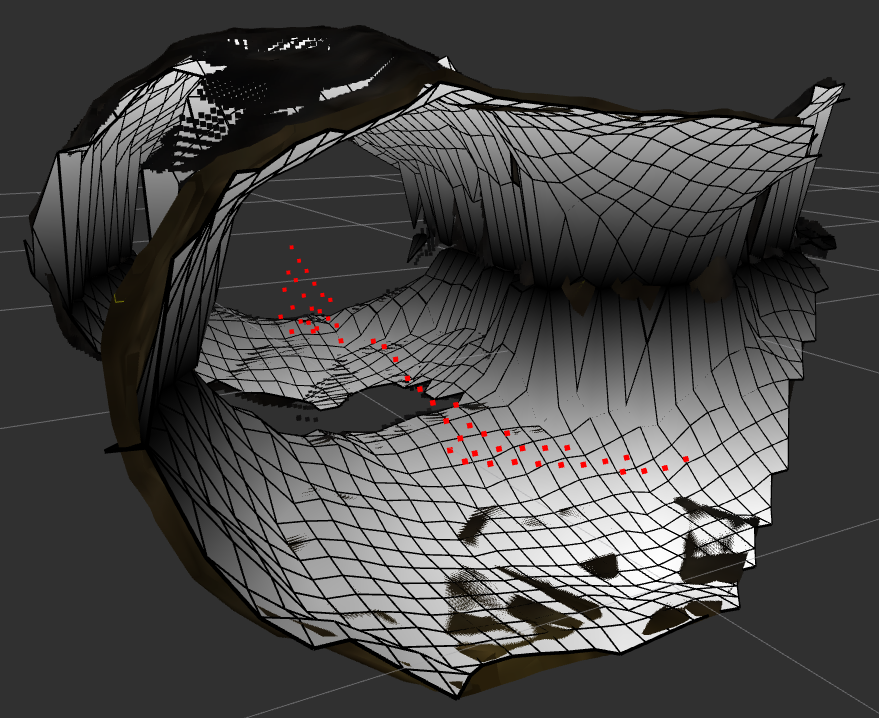
\includegraphics[width=0.5\textwidth]{posture.png}}
\caption{A live cave pointcloud, its mapped floors and ceiling, and best z-values per safe zone. }
\label{posture}
\end{figure}

The DRL-based controller was successful in learning to walk in the random noise rough terrain and random incline terrains up till the highest difficulty, but only learned to walk in the random blocks rough terrain up till 60\% of the highest difficulty. The reason for this is that the random blocks rough terrain can have discontinuities jumps in the terrain's height, which can be difficult to learn to walk in for a proprioceptive controller that cannot perceive the terrain. When the DRL-based controller was tested in the cave generated by PLUME, it was able to traverse it, but required careful teleoperation to find the right path to take. 

\begin{figure}[htbp]
\centerline{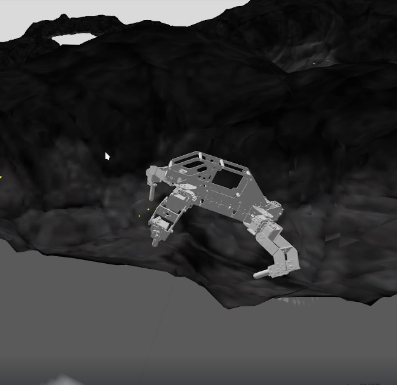
\includegraphics[width=0.5\textwidth]{example.png}}
\caption{Snapshot of the robot walking in the simulated cave. }
\label{example}
\end{figure}

The MIT Cheetah 3-like controller did not perform well in even flat terrain. The robot would not be able to lift its legs off the ground to take a step, often shuffling its feet on the ground and not making much forward progress. A suspected reason for this is that the controller uses a simplified dynamic model of the robot that assumes the robot's legs are massless, which is not the case for T-Hex. Furthermore, our modification to the foothold planning also restricts the sprawl of the robot, which could be chosen dynamically to help the robot balance itself better. 

